% **************************************************
% Document class
% **************************************************

\documentclass[
	a4paper,
	12pt,
	bibtotoc,
	listof=totoc,
	titlepage
]{scrartcl}


% **************************************************
% Settings
% **************************************************

\usepackage{settings}


% **************************************************
% Variables
% **************************************************

\newcommand*{\getUniversity}{Hochschule für angewandte Wissenschaften München}
\newcommand*{\getFaculty}{Fakultät für Geoinformation}
\newcommand*{\getTitle}{Untersuchung der Implementierung von Contraction Hierarchies in Straßennetzwerken}
\newcommand*{\getAuthor}{Daniel Holzner}
\newcommand*{\getMatriculationNumber}{26576714}
\newcommand*{\getCourse}{Geoinformatik und Navigation}
\newcommand*{\getDoctype}{Bachelorarbeit}
\newcommand*{\getSupervisor}{Prof. Dr. Thomas Abmayr}
\newcommand*{\getSubmissionDate}{\today}

% **************************************************
% Custom commands
% **************************************************
\newcommand*{\zB}{z.\,B. } % Non-breaking z.B.
\newcommand*{\dH}{d.\,h. } % Non-breaking d.h.
\newcommand*{\ua}{u.\,a. } % Non-breaking u.a.


% **************************************************
% PDF Metadata
% **************************************************

\hypersetup{
	pdftitle = \getTitle,
	pdfauthor = \getAuthor,
	pdfsubject = \getDoctype
	pdfkeywords = {Bachelorarbeit, Informatik}
}


% **************************************************
% Content
% **************************************************

\begin{document}

\titlehead{
	\begin{flushright}
		
\includegraphics[width=50mm]{logos/university_logo}
	\end{flushright}
	\begin{center}
		{\Large \getUniversity}\\
		{\large \getFaculty}
		\vspace*{10mm}
	\end{center}
}

\subject{\getDoctype\ zum Thema:}

\title{\vspace{-10mm} \getTitle}

\subtitle{Zur Erlangung des akademischen Grades Bachelor of Science}

\author{}

\date{}

\publishers{
	\parbox{\textwidth}{
		\vspace*{40mm}
		\large
		\begin{tabularx}{0.8\textwidth}{lX}
			\textbf{Vorgelegt von:} & \getAuthor \\[0.7em]
			\textbf{Matrikelnummer:} & \getMatriculationNumber \\[0.7em]
			\textbf{Studiengang:} & \getCourse \\[0.7em]
			\textbf{Betreuer:} & \getSupervisor \\[0.7em]
			\textbf{Abgabedatum:} & \getSubmissionDate \\[0.7em]
		\end{tabularx}
	}
}\normalsize

\maketitle

\begin{abstract}

\section*{Abstract}
Lorem ipsum dolor sit amet, consetetur sadipscing elitr, sed diam nonumy eirmod tempor invidunt ut labore et dolore magna aliquyam erat, sed diam voluptua. At vero eos et accusam et justo duo dolores et ea rebum. Stet clita kasd gubergren, no sea takimata sanctus est Lorem ipsum dolor sit amet. Lorem ipsum dolor sit amet, consetetur sadipscing elitr, sed diam nonumy eirmod tempor invidunt ut labore et dolore magna aliquyam erat, sed diam voluptua. At vero eos et accusam et justo duo dolores et ea rebum. Stet clita kasd gubergren, no sea takimata sanctus est Lorem ipsum dolor sit amet.

\end{abstract}

\tableofcontents

\clearpage
\listoffigures

\clearpage
\listoftables

\clearpage
\lstlistoflistings

\clearpage
\section*{Abkürzungsverzeichnis\markboth{Abkürzungsverzeichnis}{}}
\addcontentsline{toc}{section}{Abkürzungsverzeichnis}

\begin{acronym}[CI]

    \acro{CHs}[CHs]{Contraction Hierarchies}
    \acro{OSM}[OSM]{OpenStreetMap}
    \acro{PQ}[PQ]{Vorrangwarteschlange (eng. Priority Queue)}
\end{acronym}

\clearpage
\section{Einleitung}

Im Folgenden wird beispielhaft gezeigt, wie Zitate, Bilder, Tabellen oder Quellcode in die Arbeit eingefügt werden können.

\subsection{Zitate}
Menschen, die mit ihrem IQ prahlen, sind Versager (\cite[S. 99]{hawking_1999}).

\subsection{Bilder}
\begin{figure}[H]
    \centering
    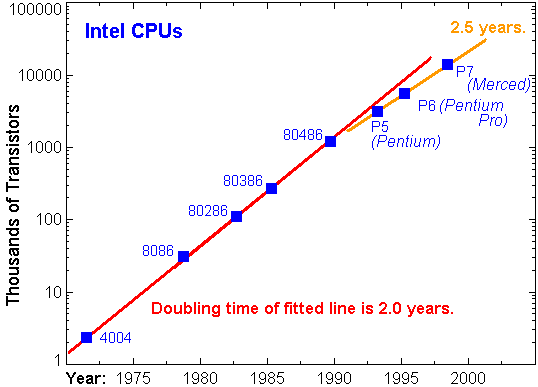
\includegraphics[width=0.5\textwidth]{figures/figure_example.png}
    \caption{Mooresches Gesetz}
\end{figure}

\subsection{Tabellen}
\begin{table}[H]
    \centering
    \begin{tabular}[H]{l|l|l}
        Bezeichnung   & Kerne & TDP   \\
        \hline
        Intel Core i5 & 6     & 111 W \\
        \hline
        AMD Ryzen 7   & 8     & 178 W \\
    \end{tabular}
    \caption{Prozessoren}
\end{table}


\subsection{Quellcode}
\begin{lstlisting}[language=java, caption=Hello World in Java, captionpos=b]
    class HelloWorld {
        public static void main(String[] args) {
            // Display the string.y
            System.out.println("Hello World!");
        }
    }
\end{lstlisting}


\clearpage
\section{Theoretische und technische Grundlagen}

\subsection{Datenstrukturen}
\subsubsection{Graph}
Um das kürzeste-Wege-Problem zu lösen, muss zunächst das reale Straßennetz in eine abstrakte Form
gebracht werden. Hierzu wird das Straßennetz als Graph modelliert. Ein Graph $G = (V,E)$ besteht aus
einer Menge von Knoten V und einer Menge von Kanten E. Jede Kante $e = (u,v)\in E$ verbindet zwei
Knoten $u,v \in V$. Ein Graph kann als gerichtet oder ungerichtet definiert werden. Bei einem
ungerichteten  Graphen sind die Kanten bidirektional und können in beide Richtungen durchlaufen
werden, während bei einem gerichteten Graphen die Kanten nur in eine Richtung durchlaufen werden
können. In dieser Arbeit wird ein gerichteter Graph verwendet, da Straßen normalerweise in einer
bestimmten Richtung befahrbar sind und damit die Richtung des
Verkehrs korrekt dargestellt wird.

Der Graph ist gewichtet, \dH für jede Kante wird während der Vorverarbeitung ein Gewicht $w(e)$
berechnet, das sich aus der Länge des Straßensegments und der maximal erlaubten Geschwindigkeit auf
dieser Straße ergibt. Der kürzeste Weg zwischen zwei Knoten ist damit der Weg mit der minimalen Zeit.

Es gibt verschiedene Möglichkeiten, einen Graphen als Datenstruktur darzustellen. Eine häufig
verwendete Darstellung ist die Verwendung von Adjazenzlisten. Dabei wird für jeden Knoten eine Liste
der benachbarten Knoten bzw. ausgehenden Kanten gespeichert. Eine andere Möglichkeit ist die
Verwendung einer Adjazenzmatrix. Dabei wird eine zweidimensionale Matrix verwendet, bei der die
Zeilen und Spalten den Knoten entsprechen. Der Eintrag an Position (i, j) in der Matrix gibt an, ob
eine Kante zwischen den Knoten i und j existiert. Ein Beispiel für einen einfachen Graph befindet
sich in Abbildung~\ref{fig:graph_ex1}.

Da wir in dieser Arbeit mit Straßennetzen arbeiten, die sehr groß sein können und Arbeitsspeicher
limitiert ist,ist es wichtig den verfügbaren Speicher effizient auszunutzen. Für den Aufbau der
\ac{CHs} und der Suche ist es außerdem wichtig schnell auf alle Nachbarn eines Knotens bzw. dessen
eingehende und ausgehende Kanten zuzugreifen. Fast alle dieser Eigenschaften erfüllt eine
Adjazenzliste, bis auf den schnellen Zugriff auf die eingehenden Kanten eines Knotens. Um das
Problem zu lösen werden in dieser Arbeit zwei Adjazenzlisten verwendet, eine für die ausgehenden
und eine für die eingehenden Kanten. Obwohl zwei Listen verwendet werden, ist der Speicherverbrauch
immer noch geringer als das Verwenden einer Adjazenzmatrix mit $O(n^2)$ Speicherkomplexität.

Es ist wichtig anzumerken, dass die Wahl der geeigneten Datenstruktur von verschiedenen Faktoren
abhängt, einschließlich der Größe und Dichte des Graphen sowie der Art der geplanten Operationen auf
dem Graphen.

\begin{figure}[H]
    \centering
    \begin{subfigure}{1.0\textwidth}
        \centering
        \begin{tikzpicture}
            \Vertices[color=gray!90!blue]{data/graphs/ex1/vertices.csv}
            \Edges{data/graphs/ex1/edges.csv}
        \end{tikzpicture}
    \end{subfigure}
    \\[3ex]
    \begin{subfigure}[b]{0.3\textwidth}
        \centering
        \begin{blockarray}{c|ccccc}
            & A & B & C & D & E \\
            \BAhline
            \begin{block}{c|ccccc}
                A &0 & 3 & 5 & 0 & 3 \\
                B &3 & 0 & 3 & 0 & 0 \\
                C &0 & 0 & 0 & 2 & 0 \\
                D &0 & 0 & 2 & 0 & 3 \\
                E &3 & 0 & 0 & 3 & 0 \\
            \end{block}
        \end{blockarray} \
        \caption{Adjazenzmatrix}
    \end{subfigure}
    \hspace{3em}
    \begin{subfigure}[b]{0.3\textwidth}
        \centering
        % \begin{blockarray}{c|ccccc}
        %     &   &   &   &   &   \\
        %     \BAhline
        %     \begin{block}{c|ccccc}
        %         A &B & C & E &   &   \\
        %         B &A & C &   &   &   \\
        %         C &D &   &   &   &   \\
        %         D &C & E &   &   &   \\
        %         E &A & D &   &   &   \\
        %     \end{block}
        % \end{blockarray} \
        \begin{blockarray}{c|ccccc}
            & A & B & C & D & E \\
            \BAhline
            \begin{block}{c|ccccc}
                A &  & $\bullet$ & $\bullet$ &   & $\bullet$ \\
                B &  $\bullet$&   &$\bullet$   &   &   \\
                C &  &   &   & $\bullet$  &   \\
                D &  &   &$\bullet$   &   &$\bullet$   \\
                E &$\bullet$  &   &   &$\bullet$   &   \\
            \end{block}
        \end{blockarray} \
        \caption{Adjazenzliste}
    \end{subfigure}
    \caption{Der oben gezeigte gerichtete Graph kann durch eine Adjazenzmatrix oder eine
        Adjazenzliste im Speicher dargestellt werden. In der Adjazenzliste wird für jeden Knoten
        eine Liste mit den ausgehenden Kanten zu den markierten Knoten abgespeichert. Die
        Zusatzinformation des Gewichts wird im Gegensatz zur Adjazenzmatrix mit der Kante
        abgespeichert.}
    \label{fig:graph_ex1}
\end{figure}

\subsubsection{Prioritätswarteschlange}




\clearpage
\section{Schlussbetrachtung}

Lorem ipsum dolor sit amet, consetetur sadipscing elitr, sed diam nonumy eirmod tempor invidunt ut labore et dolore magna aliquyam erat, sed diam voluptua. At vero eos et accusam et justo duo dolores et ea rebum. Stet clita kasd gubergren, no sea takimata sanctus est Lorem ipsum dolor sit amet. \\

Lorem ipsum dolor sit amet, consetetur sadipscing elitr, sed diam nonumy eirmod tempor invidunt ut labore et dolore magna aliquyam erat, sed diam voluptua. At vero eos et accusam et justo duo dolores et ea rebum. Stet clita kasd gubergren, no sea takimata sanctus est Lorem ipsum dolor sit amet.

\clearpage
\printbibliography

\clearpage
\begin{abstract}

\section*{Selbstständigkeitserklärung}
Hiermit erkläre ich, dass ich die vorliegende Arbeit selbstständig und ohne fremde Hilfe verfasst und keine anderen Hilfsmittel als die angegebenen verwendet habe. \\

München, den \today
\begin{figure}[H] 
  
\includegraphics[width=0.17\textwidth]{logos/signature.png}
\end{figure}

\end{abstract}

\end{document}